% ************************************************************************
%
% Introduction
%
% ************************************************************************
\chpos{22mm}{10mm}

\chapter[Introduction]{Introduction}
\markboth{\thechapter\ \ Introduction}{\thechapter\ \ Introduction}
\label{ch1:introduction}

%\mysquote{0.8\textwidth}{Quote text.}{Author (\oldstylenums{1000} - \oldstylenums{1100})}

% ************************************************************************
% sources:
% https://www.quantamagazine.org/why-the-first-drawings-of-neurons-were-defaced-20170928/
% https://www.npr.org/sections/health-shots/2017/01/26/511455876/art-exhibition-celebrates-drawings-by-the-founder-of-modern-neuroscience
% https://www.nytimes.com/2018/01/18/arts/design/brain-neuroscience-santiago-ramon-y-cajal-grey-gallery.html
% https://www.brainpickings.org/2017/02/23/beautiful-brain-santiago-ramon-y-cajal/
\section{Neuron cell reconstruction} 
\lettrine{F}{ascination} with the neuron cells dates to the moment a glance into the sample of silver-stained neuronal brain tissue over a century ago made it possible to disclose the intricate network that forms the very essence of the nervous system. The remarkable milestone drawings of Santiago Ram\'{o}n y Cajal \cite{swanson2017,ramon2008histologia} - founding father of neuroscience, remain as vivid as the images acquired by the latest fluorescence microscope and rendered with the novel computer graphics. Numerous studies \cite{ascoli2001computer,defelipe2013new,defelipe2002microstructure,defelipe1992pyramidal,van2001need,scorcioni2004quantitative,mason2007initiation,gensel2010semi} have made steps towards using physical features of the neurons to gain a deeper insight into various aspects of the functionality. Since the early hand-made illustrations depicting microscope-magnified samples of the brain tissue, the discipline gradually established as neuroscience \cite{kandel2000principles}. Furthermore, the astounding advancement of electrical engineering and computer science laid out the foundations for more specialized disciplines such as neuroinformatics and neural engineering. Recently, the attention is also directed towards brain science - domain dedicated to the investigation of the captivating mechanism of, arguably, one of the most complex and mysterious organs. The disclosure of Cajal's groundbreaking \textit{neuron doctrine}\footnote{Every neuron in the brain is separate. Neuron cells conduct information in a defined direction and communicate across the synapses \cite{glickstein2006golgi}.} brought to light the idea that the nervous system is a composite network consisting of building blocks called neuron cells that represent sophisticated, interconnected processing components that both transmit and process the information. The network structure thus matters and till large extent presents with the evidences related to the functionality.

Physical materialization of the cell portrays inner structure of the neuronal tissue and yields a valuable insight into the mechanisms behind the nervous system. Various studies have been carried out in order to understand neuron behavior and further unravel the underlying principles. Hence, the neuron morphology provides with an essential resource for specialized analysis that can typically include quantifying changes in neuronal structure caused by the external factors \cite{gomez2007immobilized,koppes2011neurite}, modeling \cite{ascoli2001computer}, classification \cite{armananzas2015towards} or the statistical analysis \cite{samsonovich2005statistical}. Widely used Sholl analysis methodology \cite{sholl1953dendritic} makes the direct use of the digital neuron reconstructions as blue print of the neuron morphology. It is commonly used in neuroscientific experimentation for quantitative analysis of the morphological characteristics of the neuron \cite{garcia2014new}. 

Numerous technical obstacles stand out when reaching out to such vastly unknown world, primarily due to the physical inaccessibility and the generally intangible nature of the whole system. Neuron cell thus represents a core building block of the brain and the nervous system. It appears in variety of shapes and specializations \cite{ascolitrees}. The estimated number of neuron cells in a human brain amounts to 89 billion \cite{herculano2009human} - number comparable to the count of stars in the Milky Way galaxy. Each neuron \textit{add: neuron dimensions} is further connected to 50 thousand other neurons on average which results in a very powerful computational network and an extremely efficient information storage. Captivating mechanism of the brain is an everlasting research topic as the complex functionality of the brain defines much of the activities, even the those such as consciousness. Discovering how the brain works is one of the grand unanswered questions of our era and central to diverse fields such as physics, mathematics, biology and recently prominent - computer science.

Nervous system activity is also manifested with the physical appearance of its neuron cells. Morphology of the single cell, shape of the neuronal network, topology or connectivity react to the external conditions or external stimuli. With the imaging tools such as fluorescence microscopy, the physical appearance the morphology of the single cell can be captured at micro meter scale can be inspected and recorded. Indeed, the studies that require deeper analysis make use of the imaging techniques that can reach nano meter scale, such as electron microscopy. In other words, accurate quantification of the cell shape is an important step towards better understanding of the cell functionality. Quantification of the neuronal structure is crucial in many neuroscience studies \cite{halavi2012digital} and quantification from microscopic images is identified as one of the major technical challenges in the digital era of neuroscience \cite{peng2015diadem}.

The advancements in informatics made it possible (Fig.~\ref{ch1__fig1}) to utilize computers to solve the neuroinformatics challenges over recent decades. With the ever growing amount of data, the processing of the information remains a challenge.   

\begin{figure}
	\begin{center}
		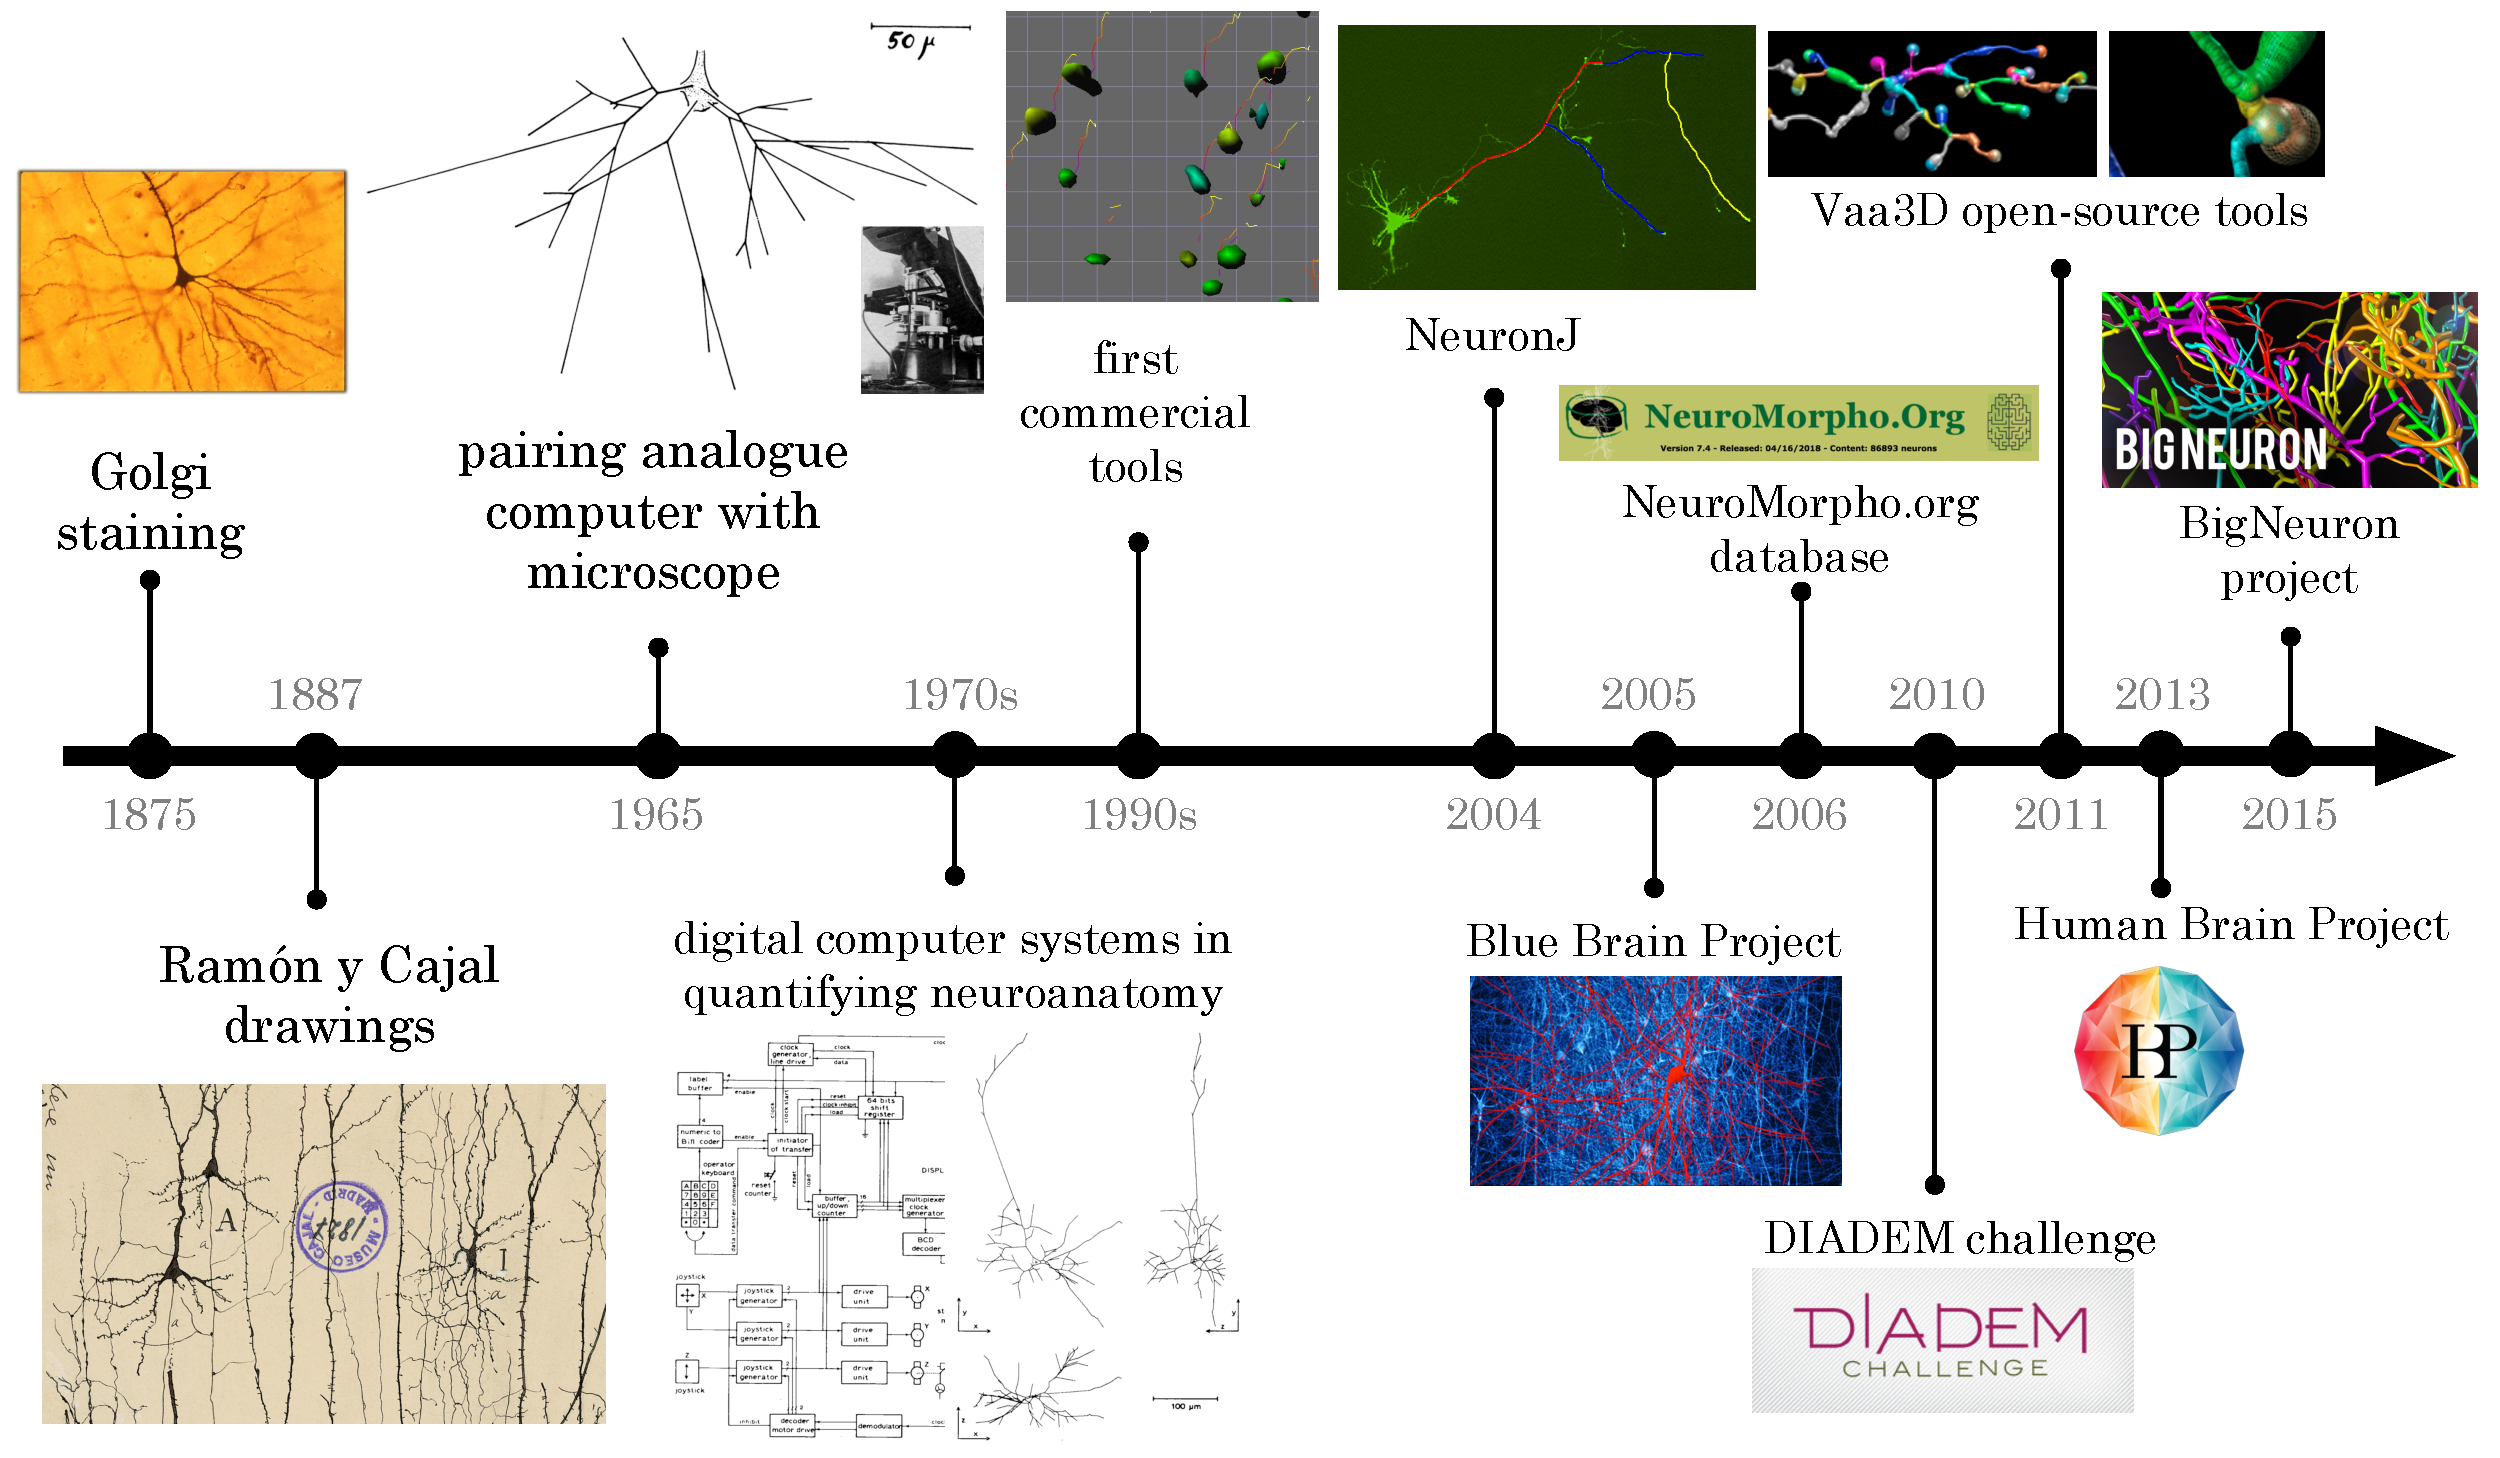
\includegraphics[width=\textwidth]{ch1_fig1}
	\end{center}
	\vspace{-3ex}
	\caption{Timeline overview of the selected keynote achievements related to the neuron morphology analysis.}
	\vspace{-1ex}
	\label{ch1__fig1}
\end{figure}

\section{Essential obstacles in neuron morphology reconstruction}
The key obstacles concerning the full, accurate and robust automation of the neuron reconstruction \cite{meijering2010neuron,donohue2011automated,acciai2016automated} can be seen through the number of factors.

\textit{Morphology} the structural ambiguities of the diverse neuron cells (Fig.~\ref{}) often intractable to the human visual comprehension.

\textit{Noise} noisy image input (imaging on the boundary of the resolution limits in case of the light microscopy). Perticles and debris erroneously detected as neuron structures.

\textit{Data size} ever increasing size of the image volume needed to be correctly processed in reasonable time. Although the processing of the 3D data (image stacks) is a  Processing of the stitched images.

\textit{Need for customization} The algorithms often need to be tailored in order to address a particular biological question and be used in wider range of the biological questions being studied which prevents them from being used across different laboratories.

\textit{Dynamic images} Analysis of the images captured from the live neuronal cultures.

Aforementioned factors impose much of the computational barrier \cite{peng2011proof,svoboda2011past} in attempt to consistently produce human-comparable digital reconstructions. The real datasets, therefore, commonly leave with the persisting need for human expert assistance to obtain the optimal output. 

\section{Neuron tracing in light microscopy images}
Neuron reconstruction tools have been adopting to the advancements of technical infrastructure available for experimentation. In decades following the emergence of neuroscience, the instrumentation has been a limiting factor to the amount and the variety of the morphologic data that could be gathered \ref{ch1__fig1}. At the beginning of the second half of the 20th century, conventional electronic analog techniques were used to join microscope and the analogue computer to automate the neuron morphology quantification \cite{glaser1965semi},  \cite{capowski1981accurate}. Variety of sowrtware platforms \cite{meijering2010neuron,acciai2016automated}. One of the key Java tools is the ImageJ library \cite{abramoff2004image} with method \cite{longair2011simple,pool2008neuritetracer}. 

\subsection{Extracting the correct tree}

\subsection{Bayesian methods in neuron tracing}

\subsection{Multiple}

\begin{figure}
\begin{center}
\includegraphics[width=0.5\textwidth]{ch1_fig2}\\
a) Shortest path tracing \\
\includegraphics[width=0.5\textwidth]{ch1_fig3}\\
b) Minimum spanning tree \\
\includegraphics[width=0.5\textwidth]{ch1_fig4}\\
c) Path-prunning
\end{center}
\vspace{-3ex}
\caption{Examples of key neuron reconstruction strategies: a) Finding optimal path between two fixed points, b) Inferring the  optimal tree structure from the given nodes c) Prunning the overcomplete neuron tree.}
\vspace{-1ex}
\label{ch1__fig2-4}
\end{figure}

Computation methods
% source:
% https://www.neuron.yale.edu/phpBB/viewtopic.php?t=3477
%Stockley, E. W.; Cole, H. M.; Brown, A. D. & Wheal, H. V.
%A system for quantitative morphological measurement and electronic modelling of neurons: three-dimensional reconstruction.
%J Neurosci Methods, 1993, 47, 39-51
%
% http://www.neuromorpho.org/myfaq.jsp (What is SWC format?)
% http://research.mssm.edu/cnic/swc.html
% http://www.neuronland.org/NLMorphologyConverter/MorphologyFormats/SWC/Spec.html
\section{Examining the neuronal reconstructions}
Once computed, neurons are typically stored in vectorized SWC format. The SWC \cite{cannon1998line,ascoli2007neuromorpho} is widely used open format for digital neuron reconstruction that describes a reconstruction as a list of 3D nodes (neuronal compartments) with seven attributes (NeuroMorpho.org):  $i$: node index identifier, node type $[0-7]$, node 3D coordinates $(x_i,y_i,z_i)$, radius $(r_i)$ and a parent node index - link towards the predecessor parent node $(j | j=-1)$ if the node has no parent soma node, Fig.~\ref{ch1__fig5}. To define a correct tree structure, each node can only have one predecessor (parent) and the parent node should have lower index so that the indexes of the reconstruction are sorted. Loops and disconnected branches should not exist. The originating node has parend  Etymologically, SWC represents the acronym containing the initials of the last names of Stockley, Wheal, and Cole. Although not directly described in their joint work on quantitative measurement and modeling of the neuron morphology \cite{stockley1993system}, the origin of the SWC name is an acronym of the initials of their last names. Moreover, there is slight uncertainty on the SWC format, especially concerning the unified definition on how soma reconstruction is addressed, resulting in several variations over the SWC standard \footnote{}.
\begin{figure}
	\begin{center}
		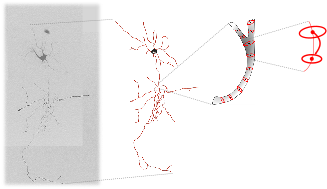
\includegraphics[width=\textwidth]{ch1_fig5} \\
		a 
	\end{center}
	\vspace{-3ex}
	\caption{Digital reconstruction of the neuron: illustration of the SWC format used to describe the idiosyncratic trr structure of the cell. Visualization using Vaa3D \cite{peng2010automatic} bioimage analysis tool.}
	\vspace{-1ex}
	\label{ch1__fig5}
\end{figure}

%\begin{figure}[t!]
%	\centering\tiny
%	\begin{tabular}{@{}c@{\hspace{0.02\columnwidth}}c@{\hspace{0.02\columnwidth}}c@{}}
%		& \hspace{3.5em}S = 2 & \hspace{3.5em}S = 3 \\[0.02\columnwidth]
%		\rotatebox{90}{\hspace{0.5em}COR = 0} &
%		\includegraphics[align=c,width=0.47\columnwidth]{synFSnrS2Cor0} & % ./fig/exp.syn/compare_snr/_F(snr,S=2,cor=0)
%		\includegraphics[align=c,width=0.47\columnwidth]{synFSnrS3Cor0} \\ % ./fig/exp.syn/compare_snr/_F(snr,S=3,cor=0)
%		\\[0.01\columnwidth]
%		\rotatebox{90}{\hspace{0.5em}COR = 1} &
%		\includegraphics[align=c,width=0.47\columnwidth]{synFSnrS2Cor1} & % ./fig/exp.syn/compare_snr/_F(snr,S=2,cor=1)
%		\includegraphics[align=c,width=0.47\columnwidth]{synFSnrS3Cor1} % ./fig/exp.syn/compare_snr/_F(snr,S=3,cor=1)
%	\end{tabular}
%	\caption{Average F score of the methods for the synthetic images as a function of SNR. Examples are shown for COR = 0 (top) and 1 (bottom) in combination with S = 2 (left) and 3 (right).}
%	\label{fig:f[snr]_synthetic}
%\end{figure}

\subsection{Measuring distances between neurons}

L-measure, neuro-blast
Distances between neurons can be based on the overlap and the inter-node metric distances.

\section{Thesis outline}
In this thesis probabilistic and bayesian methods are explored.
